\documentclass[10pt,a4paper]{article}
\usepackage[margin=1.8cm]{geometry}
\usepackage[T1]{fontenc}
\usepackage{lmodern}
\usepackage{microtype}
\usepackage{amsmath}
\usepackage{booktabs}
\usepackage{graphicx}
\usepackage{caption}
\usepackage{enumitem}
\usepackage[hidelinks]{hyperref}

\captionsetup{font=small,labelfont=bf,skip=3pt}
\setlist{itemsep=1pt,topsep=2pt,parsep=0pt,leftmargin=*}
\setlength{\parskip}{2pt}
\setlength{\textfloatsep}{8pt}

\title{\vspace{-1.2cm}\textbf{Language-Anchored, Domain-Balanced CLIP for Pedestrian Attribute Recognition}\\[2pt]
\large UPAR Challenge 2027, Track 1 (WACV 2027 Real-World Surveillance Workshop)}
\author{Muhammad Ali \quad Fasih Hasan Khan}
\date{October 2026}

\begin{document}
\maketitle
\vspace{-0.8cm}

\section{Task}
Track~1 of the UPAR Challenge asks for a model that predicts 40 binary attributes of a pedestrian from a cropped
image: age (3), gender, hair length (3), upper- and lower-body clothing length, type and 12 colours each,
and accessories (backpack, bag, glasses, sunglasses, hat). The organizers provide harmonized annotations for
Market1501, PA100k and PETA (97,669 training and 33,407 validation images). The hidden test set has 29,248 images.
Predictions are probabilities, and an attribute counts as present above a \emph{fixed} threshold of 0.5.
The ranking metric is
\[
\text{Challenge\_Avg} = \frac{2\,\text{mA}\cdot\text{F1}_\text{inst}}{\text{mA}+\text{F1}_\text{inst}},\qquad
\text{mA} = \frac{1}{40}\sum_k \tfrac{1}{2}\left(\text{TPR}_k+\text{TNR}_k\right),
\]
computed per dataset and then averaged. Submissions are \emph{code}: a \texttt{run.py} executed in a fixed Docker
image (PyTorch 2.4.1, an NVIDIA A10 GPU, no network) with a 5-minute limit. We trained on a single RTX 3060\,Ti (8\,GB).

\section{Method}
\textbf{Backbones.} Model~A is ConvNeXt-T (ImageNet weights). Model~B is the CLIP ViT-B/16 image encoder (OpenAI weights,
QuickGELU) at $256\times128$ input, with its positional embedding interpolated to the $16\times8$ patch grid.
Model~C is CLIP ViT-L/14. To fit 8\,GB it sees $224\times112$ (resized inside the network), its lower 12 of 24 blocks are frozen and gradient
checkpointing is on (4.6\,GB peak). Training uses AdamW (backbone learning rate $3\cdot10^{-5}$ with layer-wise decay 0.7, head
$10^{-3}$), a cosine schedule with warm-up, mixed precision, EMA weights (decay 0.999) and a positive-rate-weighted
BCE loss. The best epoch is selected on the validation protocol. On top of the backbones we added five components:
\begin{enumerate}[label=\textbf{N\arabic*}]
\item \textbf{Language-anchored head.} $z_k = s\cdot\cos(f,w_k)+b_k$, where $w_k$ is initialised from CLIP text embeddings of
attribute prompts (positive minus negative prompt) and $b_k$ from training positive rates. Zero-shot, this head
already scores 0.638 (ViT-B) against 0.530 for the organizers' prior-only baseline.
\item \textbf{Domain-balanced sampling.} Each dataset supplies a third of every epoch, because the metric weights datasets equally.
\item \textbf{Surveillance degradation augmentation.} With probability 0.3: down/up-scaling, JPEG compression, blur,
brightness/contrast changes and random erasing.
\item \textbf{Protocol-matched calibration.} Because the 0.5 threshold is fixed, we learn one global logit offset $\delta_k$ per
attribute by coordinate ascent on the exact metric (per dataset, then averaged). The offsets are fitted on one half of val,
shrunk by a factor $\lambda$ chosen on the other half, refitted on all of val, and built into the exported model.
\item \textbf{Structure-aware decoding.} For (near-)exclusive groups (age, upper/lower colour), if no member exceeds 0.5,
the arg-max is lifted above 0.5. A group is decoded this way only if that improves the held-out score.
\end{enumerate}
\textbf{Inference.} The submission is a single fp16 TorchScript module that takes uint8 images and contains normalisation,
offsets, sigmoid and decoding. \texttt{run.py} decodes JPEGs on 16 threads and overlaps decoding with GPU work.
On the platform, sub03 processed all 29,248 test images in 34.8\,s.

\section{Evaluation}
We use the official val split with the test protocol (per-dataset metric, averaged). Calibration is fitted on val,
so for N4/N5 we report a \emph{held-out} score (2-fold: fit on one half, score the other).

\begin{table}[h]
\centering\small
\begin{tabular}{@{}lccc@{}}
\toprule
Model & val, offsets$=0$ & val held-out (+N4+N5) & \textbf{test} \\
\midrule
Organizers' prior-only baseline & 0.530 & -- & -- \\
CLIP ViT-B/16 zero-shot (N1 head, no training) & 0.638 & -- & -- \\
A: ConvNeXt-T, N2+N3, flip-TTA & 0.8452 & 0.8569 & -- \\
\textbf{B: CLIP ViT-B/16, N1--N5 (sub03)} & 0.8574 & 0.8742 & \textbf{0.7699} \\
C: CLIP ViT-L/14, N1--N5 (sub06) & 0.8582 & 0.8730 & not scored$^\dagger$ \\
B+C ensemble, logit weights 0.4/0.6 (sub07) & 0.8625 & \textbf{0.8803} & not scored$^\dagger$ \\
\bottomrule
\end{tabular}
\caption{Main results (Challenge\_Avg). $^\dagger$Built and validated, but not scored because of the platform outage (Section~\ref{sec:outage}).}
\label{tab:main}
\end{table}

\begin{table}[h]
\centering\small
\begin{tabular}{@{}lcc@{}}
\toprule
Change to the full recipe (2-epoch CLIP ViT-B/16, held-out 0.8709) & held-out & effect of component \\
\midrule
N1: random head instead of text-initialised & 0.8675 & $+0.0034$ \\
N2: natural sampling instead of equal per dataset & 0.8665 & $+0.0044$ \\
N2 variant: sampling $\propto\sqrt{\text{dataset size}}$ & 0.8694 & $-0.0015$ vs.\ equal \\
N3: no degradation (clean val / degraded val, $0.4\times$ scale + JPEG q40) & 0.8717 / 0.8605 & $-0.0008$ / $+0.0060$ \\
N4: no calibration (full Model~B) & 0.8575 & $+0.0167$ \\
N5: no structured decoding & -- & $+0.0001$ to $+0.0007$ \\
\bottomrule
\end{tabular}
\caption{Ablations. N3 does not help on clean val, but on degraded val it is worth 0.6 points.}
\label{tab:abl}
\end{table}

\begin{figure}[!htb]
\centering
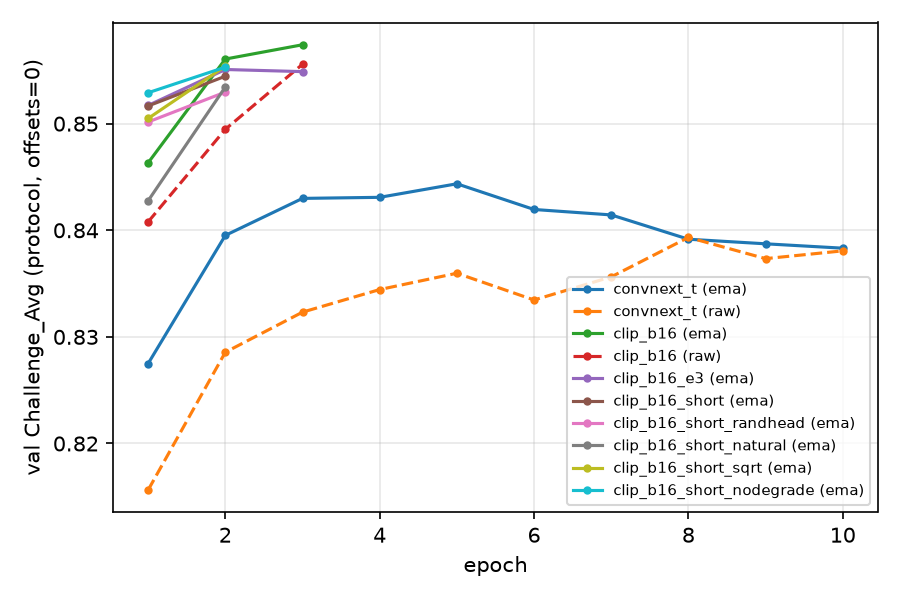
\includegraphics[width=0.335\linewidth]{figures/val_curves.png}\hfill
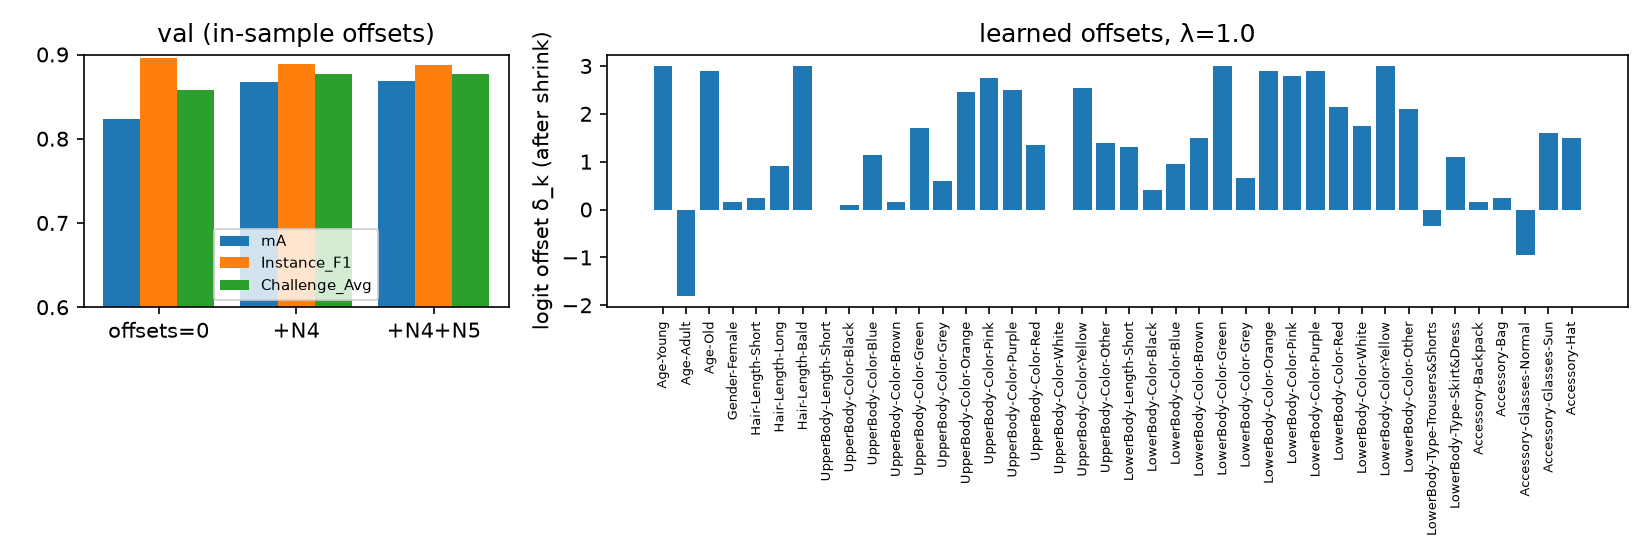
\includegraphics[width=0.655\linewidth]{figures/calibration_clip_b16.png}
\caption{Left: val Challenge\_Avg per epoch. CLIP overtakes ConvNeXt after one epoch and peaks at epoch 3, while
Market1501 starts to overfit. Right: effect of N4 and N5, and the learned offsets of Model~B. Many offsets hit the $+3$ cap for rare colours.}
\label{fig:curves}
\end{figure}

\textbf{Test result.} sub03 (Model~B) scored \textbf{0.7699} Challenge\_Avg on the hidden test set (mA 0.7725, instance F1 0.7672),
47th of the 50 listed entries. First place has 0.8021, and about 30 teams lie within 0.795--0.802 (Appendix~\ref{sec:proof}).

\section{Additional models and the platform outage}\label{sec:outage}
After sub03 we built four more packages, all validated with our local ingestion simulator:
\textbf{sub05} (Model~B retrained on train+val), \textbf{sub06} (ViT-L/14), \textbf{sub07} (the B+C ensemble, best held-out score 0.8803)
and \textbf{sub08} (the ensemble with both members retrained on train+val).
None of them received a test score. The platform's logs show that sub05's prediction step completed on 20~Oct
(29,248 images in 46\,s), but scoring never started and the submission stayed ``Running''. sub07 was uploaded on 21~Oct
at about 13:40~UTC. From about 13:45~UTC, \texttt{codabench.org} stopped responding (other sites remained reachable),
and it was still unreachable after the phase closed on 22~Oct at 12:00~UTC. Our only scored submission is therefore sub03.
The Codabench queue was also stalled for several hours on 20~Oct, so our first upload of sub03 had to be cancelled and re-submitted.

\section{Challenges}
\begin{itemize}
\item \textbf{Large val-to-test gap} ($0.874\rightarrow0.770$). The test set is a different domain. PETA's val split probably shares
identities with train, which makes val optimistic. The N4 offsets, fitted on val, saturate at $+3$ for rare colours (Fig.~\ref{fig:curves}),
so they may over-predict those attributes on new data.
\item \textbf{Overfitting to Market1501.} Equal sampling shows its 10k training images about 3.3 times per epoch. Market1501 val fell every epoch
after the first (0.835$\rightarrow$0.820), so both CNN and CLIP runs had to be stopped early.
\item \textbf{Compute.} One 8\,GB GPU made ViT-L/14 possible only with frozen lower blocks and gradient checkpointing (about 20\,min per epoch).
A slow connection made downloading data and weights take hours.
\item \textbf{Platform reliability.} Queue stalls, a submission that was never scored, and finally the site going down near the deadline.
\end{itemize}

\section{Possible improvements}
\begin{itemize}
\item \textbf{Calibrate for transfer, not for val.} Fit offsets leave-one-dataset-out, cap or shrink them more strongly ($\lambda<1$),
and test sub04 ($\lambda=0.5$) against sub03 on the leaderboard.
\item \textbf{Stronger domain generalization.} Heavier colour and style augmentation, mixing datasets in a batch,
and sampling proportional to dataset size, which scored best on Market1501 and PA100k.
\item \textbf{Bigger, ensembled models.} Fully fine-tune ViT-L/14 on a larger GPU, and use ensembles: B+C gained $+0.006$ held-out,
and ensembles usually hold up better on new domains.
\item \textbf{Use the val data for training} (allowed by the rules). sub05/sub08 do this but could not be scored.
\end{itemize}

\textbf{Code.} Training, calibration, export, an ingestion simulator, all configs, logs and figures are in the repository
(\texttt{src/}, \texttt{configs/}, \texttt{tools/}, \texttt{results/}). The README lists the commands to reproduce every model.

\appendix
\section{Proof of submission}\label{sec:proof}
\begin{itemize}
\item Codabench competition 18180 (Evaluation Phase), account \texttt{ali123}.
\item Submission \textbf{1004948}, file \texttt{sub03\_clip\_b16\_calib.zip}: status \emph{Finished}, Challenge\_Avg \textbf{0.7699}.
\item The same package was also submitted from the second member's account (\texttt{fasihhk}, submission 1005565), with identical scores.
\item The platform's run logs and the API record are in \texttt{deliverables/\allowbreak proof\_of\_submission}.
\end{itemize}
\begin{figure}[h]
\centering
\IfFileExists{../proof_of_submission/sub03_screenshot.png}{%
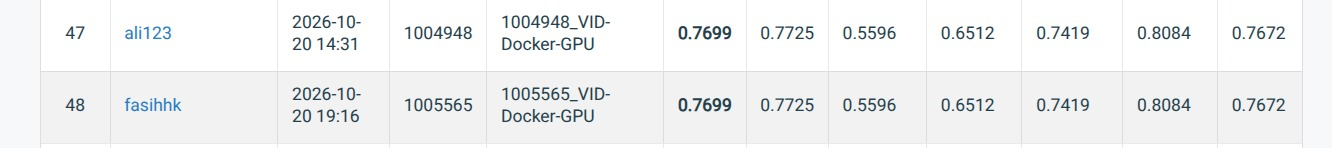
\includegraphics[width=\linewidth,height=7cm,keepaspectratio]{../proof_of_submission/sub03_screenshot.png}}{%
\fbox{\parbox{0.8\linewidth}{\centering\vspace{1cm}Screenshot: \texttt{proof\_of\_submission/sub03\_screenshot.png}\vspace{1cm}}}}
\caption{Codabench leaderboard (Track~1 test set): our sub03 entries at positions 47 (\texttt{ali123}) and 48 (\texttt{fasihhk}).}
\end{figure}

\end{document}
